\documentclass[conference]{IEEEtran}
\usepackage[colorlinks=true]{hyperref}
\usepackage[usenames,dvipsnames,svgnames,table]{xcolor}
\usepackage{array}
\usepackage{graphicx}
\newcommand{\subparagraph}{}
\usepackage{titlesec}
\titleformat{\section}{\color{brown}\normalfont\bfseries}{\color{black}\thesectiondis}{1em}{}
\titleformat{\subsection}{\color{brown}\normalfont\bfseries}{\color{black}\thesubsection}{1em}{}
\titleformat{\subsubsection}{\color{brown}\normalfont\bfseries}{\color{black}\thesubsubsection}{1em}{}
\hyphenation{op-tical net-works semi-conduc-tor}
\begin{document}
\title{MUD: Simple, Effective IoT Network Security}
\author{\IEEEauthorblockN{Steven Rich}
\IEEEauthorblockA{Cisco Systems, Inc.\\
170 W. Tasman Dr.\\
San Jose, California 95134\\
Email: srich@cisco.com}
\and
\IEEEauthorblockN{Thorsten Dahm}
\IEEEauthorblockA{Google Inc\\
1600 Amphitheatre Parkway\\
Mountain View, CA  94043\\
Email: thorstendlux@google.com}
}

\maketitle

\begin{abstract}
Manufacturer Usage Descriptions, or MUDs, allow a manufacturer to
cheaply and simply describe to the network the accesses required by an
IoT device without adding any extra cost or software to the devices
themselves.  This document describes the lifecycle of Manufacturer
Usage Descriptions (MUDs) by describing detailed MUD scenarios from
the perspective of manufacturers.
\end{abstract}

\section{First, a Story}
{\it This is a fictional account of {\rm Acme Lightbulb and Sensor}'s
  first foray into developing and delivering IoT-connectable devices,
  having been a trusted developer of traditional, non-connected
  lighting technology for decades.}

The quarter-over-quarter numbers were looking better than expected.
The impact that the new ``Acme LightTheWay'' smart lightbulbs were
having on the bottom line was extraordinary.  Acme had taken a gamble
by using investment-grade power modules with operating margins that
would insure long lifetimes and high customer satisfaction as a means
to differentiate and develop brand loyalty.  The online forums picked
up on it and word had spread: Acme bulbs were the ones to buy.  Yes,
they were slightly more expensive at first (but not by much), but they
paid for themselves and then kept on doing so long after the cheap
ones had blown out their under-spec'd capacitors.  Moreover, the
cloud-based controller with smart phone app was a user-experience
success, managing to please customers broadly by giving the features
that they wanted while still being simple to use.

The reports of the DDoS attacks started to hit the mainstream media
outlets during prime time on the East Coast of the U.S.  Something was
going on against a couple of major infrastructure players that had
disabled critical components of the internet, affecting BGP, DNS, and
NTP.  Details were sketchy, but as network operators started getting
notified that their networks were the sourcing attack traffic, things
got more confusing: some of the biggest sources of DDoS traffic had no
appreciable computing systems that could generate the volumes of
traffic being seen.

Netflow analyses were studied, and the picture began to form: it was
another IoT-based DDoS attack.  By the time the sun had set on the
West Coast, the affected equipment was starting to be called out by
name.  One of the first to be identified as the ``Acme LightTheWay''.
Their successful product launch had guaranteed a large deployment.
Their excellent hardware had meant that many were still in service and
operating perfectly.  Unfortunately for them, the software agent
running on the bulbs had an obscure flaw, and one that they themselves
at Acme had not even written: it had come in with the inclusion of a
commonly-used open source, third-party library.

They weren't the only ones using it, and they weren't the only ones
named in the current attack.  But the damage had been done.  The scale
of the attack, the unfortunate prominence of their name in the
reporting, and the speed at which the attack had escalated had
everyone talking about them in all the wrong ways.  Tactical
remediation was put into place as quickly as possibly by all of the
network operators.  Network access was restricted to the cloud servers
when possible, but many simply blocked all external network access in
the cases in which the bulbs had been provisioned to a ``light bulb
vlan''.

How could this have been avoided?  Could it have been?  The answer is:
{\em yes}.  Using MUD, the network could have been automatically
configured to be in the same state of security almost as soon as the
light came on, with full functionality.  And the bulbs and other IoT
devices like it would have been locked down to the minimal, sensible
network access specified by Acme from the start, eliminating the
devices' abilities to attack other devices.

\section{MUD Motivation}
As the anecdote above showed, the addition of IoT devices to a network
can, at least theoretically, expand the attack surface of that
network.  Even if a device does not have exploitable vulnerabilities
(in the sense of an attacker injecting and running malware on it), it
may be susceptible to denial-of-service (DoS) attacks and thus could
have its functionality impaired by attackers.  Recent events have
shown just how real, and not just theoretical, such attacks can be.

A detailed summary of the current state of understanding of the Mirai
botnet's use of IoT devices can be found in
\href{https://www.flashpoint-intel.com/action-analysis-mirai-botnet-attacks-dyn/}{this
article}.  It is estimated that around 100,000 IoT devices generated
more than a terabit per second of DDoS traffic.

Also consider the
\href{http://www.pcworld.com/article/3147311/security/backdoor-accounts-found-in-80-sony-ip-security-camera-models.html}{Sony
Cameras IP Security} article which describes a vulnerability in many
camera models which could be exploited to launch attacks like those
seen in the
\href{http://www.pcworld.com/article/3134056/hacking/an-iot-botnet-is-partly-behind-fridays-massive-ddos-attack.html}{massive
DDos attack on DynDNS}.  As both of these incidents show, more
network-accessible devices which can connect to arbitrary external
addresses can, if those devices permit too much access or if they have
vulnerabilities which allow arbitrary code execution, be used by
attackers to amplify attacks and to do so by using origin addresses
spanning broad ranges of networks.

Concerns about the negative possibilities of attacks related to IoT
devices is also discussed in
\href{https://www.technologyreview.com/s/603015/security-experts-warn-congress-that-the-internet-of-things-could-kill-people/}{this
article} in the MIT Technology Review
that also discusses some of
the regulatory and government angles in play.  In a recent move, the
U.S. Federal Government has taken the step of
\href{https://www.cnet.com/news/d-link-lawsuit-ftc-security-hackers/}{suing
  D-Link}, accusing it of ``poor security practices'' for some of its
IoT devices.

MUD provides a much more light-weight model of achieving very
effective baseline security for IoT devices by simply allowing a
network to automatically configure the required network access for IoT
devices so that they can perform their intended functions without
granting them gratuitous, unrestricted network privilege.

\section{MUD Introduction}
Manufacturer Usage Descriptions (MUDs) provide advice to end networks
on how to treat specific classes of devices.  The MUD architecture is
explained in \cite{I-D:ietf-opsawg-mud}, but we will describe it
briefly here and also discuss details where necessary to understand
this document.  At its most basic, MUD is a system by which the IoT
device itself tells the network exactly how to retrieve its network
access requirements (in a ``MUD File''), and network infrastructure
can fetch and act up this information.  The MUD File itself is a
static text file\footnote{The HTTPS server(s) which serves up the file
  or files can technically use whatever technology for implementation
  that is desired.  However, each MUD file may simply be stored and
  served up as simple, single text files.} which the network
infrastructure element responsible for it can retrieve from the
manufacturer or from whomever the manufacturer delegates the
responsibility to.

To ``add a MUD file specification'' to an IoT device is a very minimal
change.  To whatever dynamic network registration protocol which is
currently being used by the device (e.g. DHCP, etc.), the URL for the
MUD file is added.  It is so simple that the device manufacturer can
compile the URL into the firmware of the device, assuming that that is
the most appropriate implementation.\footnote{A lightbulb, for
  example, may comprise a microcontroller with embedded flash and
  essentially no bulk storage, so the URL can be compiled directly
  into the data section of the software image.}  The essential point
is that MUD does not force a large behavioral change on the IoT device
itself, and the serving up of the MUD file during the lifetime of the
devices is similarly relatively low-impact.  The bulk of the
complexity of MUD is concentrated within the network elements which
perform operations to retrieve the MUD files, possibly cache them, and
then configure the network in response, but even there, the network
elements effected mostly already perform all of these actions, albeit
not automatically in most cases.

For this description, one can consider three general
classes of actors in the MUD ecosystem:
\begin{itemize}
\item Device manufacturers
\item Networking equipment manufacturers
\item Network operators
\end{itemize}

Note that end users are not mentioned here, as their involvement in
MUD is minimal at best (and likely only present in the simplest of
deployments).  Note also that ``Device manufacturers'' are described
with the assumption that they will both include MUD URIs within their
devices as well as service MUD URI queries (via a cloud service or via
their own web infrastructures).  It is possible that a manufacturer
will delegate the MUD URI response function to a third party.  The
question of who actually services network requests for the MUD URI is
an administrative one and does not affect the MUD architecture.  It
does give device manufactures more flexibility, though, in managing
their investment into the MUD ecosystem.

This document will describe the MUD ``lifecycle'' from the standpoint
of manufacturers, but it is also intended to be informative to persons
interested in standardization, installation, or other areas where MUD
may be in play.  Where appropriate, suggestions of best practices will
be given if there are no specific hard requirements.

\section{Terminology}

Before going into descriptions how MUD works, we will list terms used
within the MUD ecosystem:

\begin{description}
\item[{\color{brown}\it MUD}] \hfill \\ Manufacturer Usage Description
\item[{\color{brown}\it MUD file}] \hfill \\ a file containing YANG-based JSON that
  describes a recommended behavior
\item[{\color{brown}\it MUD file server}] \hfill \\ an HTTPS server that hosts a MUD file
\item[{\color{brown}\it MUD controller}] \hfill \\ the system that requests and
  receives the MUD file from the MUD server.  After it has processed a
  MUD file it may direct changes to relevant network elements
\item[{\color{brown}\it MUD URL}] \hfill \\ a URL that can be used by the MUD
  controller to receive the MUD file
\item[{\color{brown}\it IEEE 802.1AR}] \hfill \\ A IEEE specification for a
  certification-based approach for communicating device
  characteristics
\item[{\color{brown}\it URL}] \hfill \\ Universal Resource Locator
\item[{\color{brown}\it YANG}] \hfill \\ A data modeling language for the
  definition of data sent over the NETCONF network configuration
  protocol\cite{ietf:rfc-yang}
\item[{\color{brown}\it NETCONF}] \hfill \\ Network Configuration
  Protocol\cite{ietf:rfc-netconf}
\item[{\color{brown}\it JSON}] \hfill \\ Javascript Object Notation, a human- as
  well as machine-readable file format containing textual
  representations of ``objects'' such as strings of characters,
  numbers, boolean values, and lists and dictionaries of such objects
  and collections of objects
\item[{\color{brown}\it CDN}] \hfill \\ Content Distribution Network,
  a service which allows content providers to push content out to
  points in the network much closer to consumers.  Akamai, CloudFlare,
  and Rackspace are just a few examples of commercial CDNs, and most
  telcos also provide CDN services.
\end{description}

Many of these terms are in common usage with the IETF or other network
standards bodies and are thus used for consistency.  More information
about terms like ``URL'', ``URI'', ``YANG'', and ``NETCONF'' can be
found in the standards and references published by the IETF and others.

\section{MUD Overview}
A full description of MUD is given in \cite{I-D:ietf-opsawg-mud}.  In
short, when a device such as an IP-enabled lightbulb is connected to
the network and given power, that device will perform some action to
acquire a network identity, including an IP address, such as by making
a DHCP request.  If that request has a MUD URI in it, equipment in the
network (not necessarily the DHCP server) can use that URI to retrieve
the device's MUD file from the MUD file server.  Some other networking
component (the switch to which the bulb in connected, for example) can
then act on the contents of the retrieved MUD file and apply the
appropriate configurations to allow the device to function normally
while restricting where it can connect.

A MUD file's contents will mostly contain descriptions of which
protocols are required by the device and over what port or ports.

From the perspective of a manufacturer, the essential elements to note
are the following:
\begin{enumerate}
\item On the device itself, the only change required to add MUD
  compliance/functionality is to add a field populated with a URI to
  whatever network access protocol is already being used (i.e., DHCP,
  IPv6 AD, etc.).  This will be a static text string which will
  probably remain constant throughout the life of the product and
  which is identical for every instance of a product run (i.e., there
  is no per-serial-number version of the MUD URI)
\item The MUD file which is to be returned via an HTTPS server can be
  a static file and can be reused for devices which have the same
  network access requirements.  The service which returns the MUD file
  will not be responsible for any security policy enforcement, as that
  is the job of the network which contains the devices themselves
\item MUD files are fairly short (on the order of tens of lines of
  text) and are thus trivial to serve either directly or via a CDN
\item The act of retrieving the MUD file and of acting on it is
  entirely up to the network infrastructure and not a responsibility
  of the IoT devices themselves.  MUD does not impose any behavioral
  requirements on the IoT devices themselves other than that they must
  send the MUD URI during network access configuration, as mentioned
  earlier
\end{enumerate}

How does MUD work in practice?  Figure~\ref{fig:MUDNetwork} on
Page~\pageref{fig:MUDNetwork} shows a
representation of the high-level MUD information flow.
\begin{figure*}
  \begin{center}
    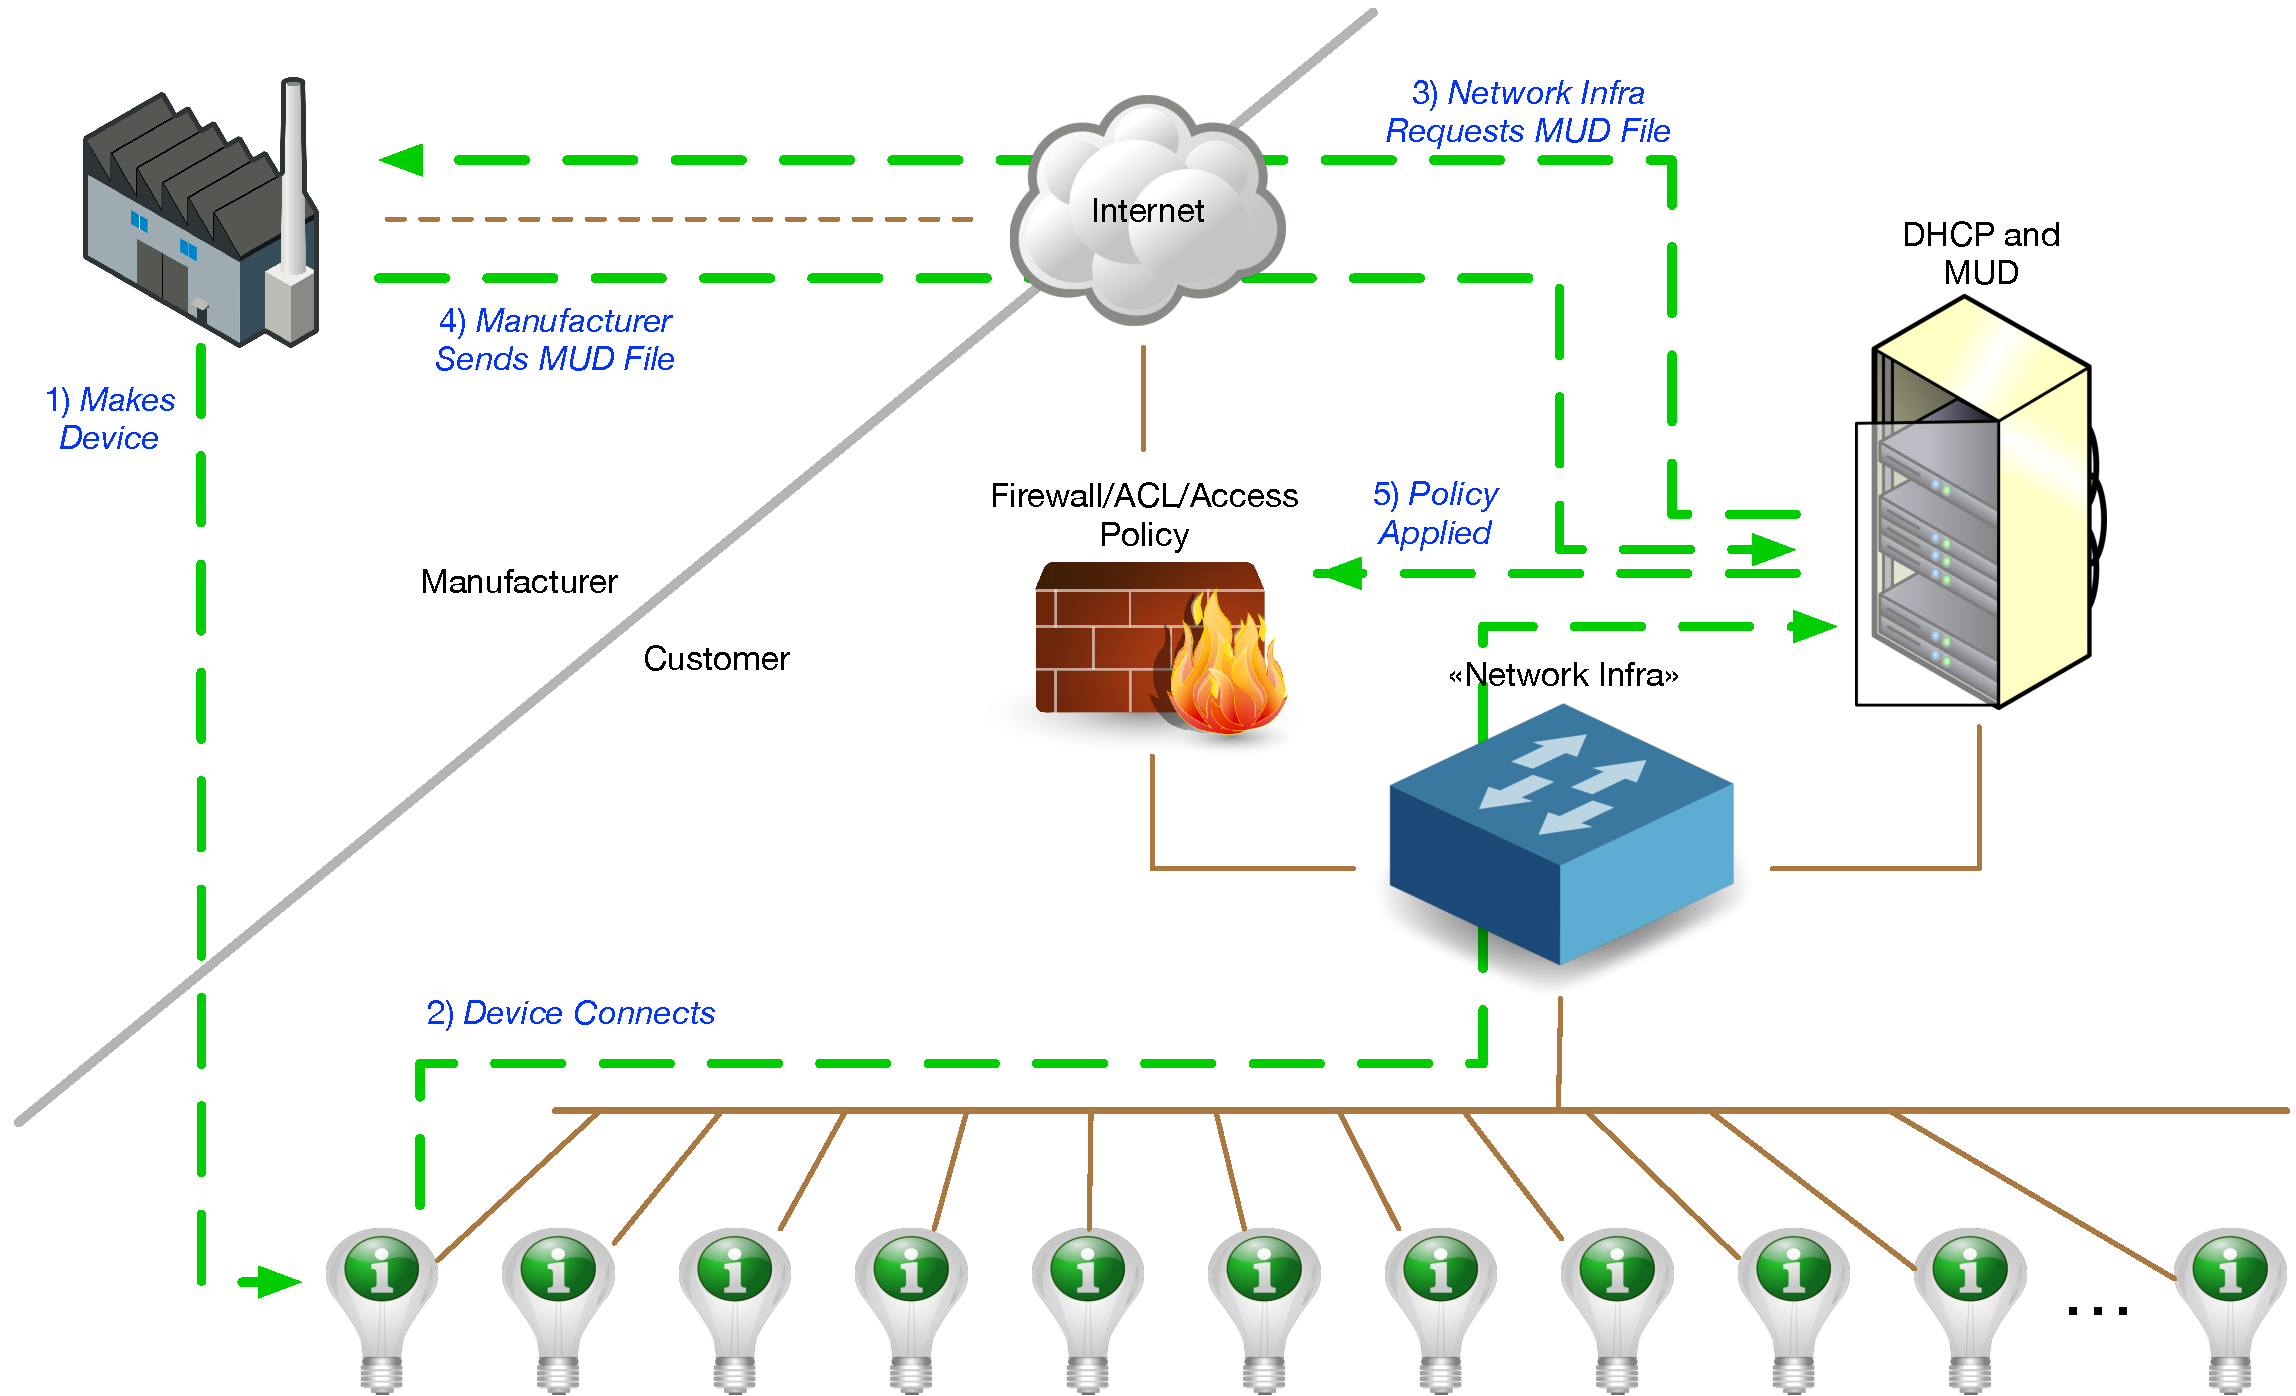
\includegraphics[width=\textwidth]{Graphics/MUDNetworkFlow}
    \caption{MUD High-level information flow}
    \label{fig:MUDNetwork}
  \end{center}
\end{figure*}
This document deals almost exclusively with elements in the upper left
of that figure.  Specifically, it describes what a manufacturer should
do to put a MUD file into a device and what is required for a
manufacturer (or a designee of the manufacturer) to answer requests
for MUD files from network operators whose networks provide
connectivity for such devices.


\section{Device Manufacturer Considerations}
The device manufacturers have the most insight into what resources the
devices will need once they are installed in a network.  They are thus
best-suited to author the network profiles which will be required by
the devices that they make for correct operation.  Conversely, each
manufacturer cannot know what each network's other requirements happen
to be.  As a result, the manufactures should provide configuration
requirements for their devices which network operators can apply in a
way best suited for their networks.  The network operator can optimize
operations through caching, LAN segregation, etc., and can use the MUD
information to further secure the network.

If a manufacturer makes many devices which have similar network access
requirements, that manufacturer may want to leverage common profiles.
They should do so only when the profiles are truly close enough to be
treated as the same.

Device manufacturers have three responsibilities under MUD:
\begin{itemize}
\item They must author a MUD profile which describes a device's
  requirements for network access
\item They must encode a MUD URI into the device such that when the
  device performs DHCP or similar, the networking infrastructure is
  informed and can fetch and act on the MUD profile
\item The manufacturer (or someone to whom the manufacturer has
  delegated the responsibility) must service requests to fetch the MUD
  profile(s) via an HTTP GET request
\end{itemize}
Since the MUD profiles can be static files, there is very little
overhead required to serve these profiles.  Due to their static
nature, they are inherently cacheable and could also suitably be
served via a content distribution network (CDN).

Similarly, since the URI can be essentially static (the actual device
configurations are easily updatable since they are contained in the
MUD file, not the URI), the manufacturer can assign a name space and
begin encoding the URIs into the devices relatively early in the
manufacturing process.  An important point is that manufacturers
should adopt and follow a nomenclature that insures that they can
sufficiently distinguish classes or families of devices with different
requirements and assign them different URIs.  From a security
standpoint, it is better to have several URIs with more granular
security profiles than it is to have a very few URIs with "catch-all"
(and thus more open) security profiles.  This ensures that a customer
using a single family of devices will have the most closed network
configuration possible.

If the device manufacturer decides to update the profile, then it may
do so at any time, independently of updates to the firmware on the
devices themselves.  If it is expected that a profile may change
frequently (say, for a new class of devices which aren't fully
understood yet), then the MUD profile for said device should have a
fairly short TTL (as compared to a device with a well-known network
access profile).

\section{High-level MUD Lifecycle}

The following lifecycle description is described considering a single
device.  As additional devices are added to a portfolio, the same
steps are taken for each one where necessary.  Each step can be
isolated or coordinated with other device instances where convenient.
There is little coupling inherent in the way that the various phases
of MUD deployment operates to impose strict requirements in this area.

\begin{enumerate}
\item Based on a device's function, a MUD profile is either:
  \begin{itemize}
  \item Chosen from a library of existing profiles for similar devices
    
  \item Written anew to describe this device's network requirements
  \end{itemize}
\item If the profile is pre-existing, the a choice is made if this
  device will receive a new URI or if it should be classed as
  identical to existing devices and use the same URI
 
\item The chosen URI is assigned to the device so that when the device
  performs network initialization, the URI is included in the request
  (i.e., DHCP, ANIMA, etc.)
 
\item In parallel or in advance (but prior to first customer
  shipment), the device manufacturer should allocate in an appropriate
  namespace and place the MUD profiles for when the URI is used as a
  URL.
 
\item The MUD profile should be made available to customers until such
  a time that the device is unsupported.  While it is outside the
  scope of this document, The manufacturer should support MUD profile
  retrieval for each device for at least as long as the manufacturer
  supports the devices themselves, or at least arrange for some
  content provider to do so (such as a CDN).

\item If the profile is found to contain an error, the manufacturer
  should update the profile.  Devices which are already deployed will
  continue to use the original URI (unless a firmware updates changes
  it), so the original profile should be corrected
 
\item If a device manufacturer chooses to update a MUD-enabled
  device's firmware, the manufacturer may update the MUD URI to a new
  one.  The manufacturer should change the URI if the network access
  requirements of the new firmware are sufficiently different from
  those of the original firmware version.
\end{enumerate}


\section{MUD URL}

The MUD URL is a very visible and important part of MUD that is best
done correctly from the start, for once it is embedded in an IoT
device, changing it for the fielded devices will be, at best,
inconvenient.  Choosing a scheme for organizing the ``name space'' for
the portion of the URL which is controlled by the device manufacturer
may have knock-on effects such as the URL GET request routing behavior
that must be supported during MUD file retrieval.

The format of the URL is:

\begin{center}
  \ttfamily\scriptsize
  https://{\em authority}/.well-known/mud/{\em mud-rev}/{\em model}
\end{center}
and may be post-fixed with ``{\ttfamily\small ?{\em extras}}''.
Referencing \cite{ietf:rfc3986}, the {\em authority} element is
described by the ``authority'' type, the {\em model} element by the
``segment'' type, and {\em extras} by the ``query'' type.  This gives
considerable flexibility to manufacturers to structure their various
namespaces to handle a huge variety of device types.  To convey a
sense of the possibilities, this section will describe some possible
URI namespace designs which could be used for a fictional line of
devices manufactured and sold by the fictional ``Acme Lightbulb and
Sensor'' company.

The fictional product line will include lighting, lighting control,
fan control, temperature sensing, motion sensing, and controllers.
The device families are broken into two broad categories:
\begin{enumerate}
\item Cloud-based
\item Local controller-based
\end{enumerate}
The cloud-based devices will need to ``phone home'' to Acme's
internet-facing cloud service points.  These service points will be
addressable via a stable DNS name as a REST interface.  The local
controller-based devices will need to perform similar network
connections as those of the cloud-based devices, but instead of
accessing a cloud resource, the devices will need to access a
controller (or controllers) which reside on the local network.  (The
address of this controller will be discovered via other means such as
a DHCP response, a retrieved configuration, mDNS, or other means.)

The manufacturer can choose two radically different strategies for
designing the namespace of their URIs.  They can use a human-readable
format which is self-documenting and will thus be pleasing to network
operators who will have to troubleshoot networks.  As an alternative,
the URI {\em model} element can be some unique-per-device-class
identifier which is itself otherwise non-descript.  While this is
technically possible, it becomes cumbersome since it offers no insight
into what purpose the MUD file to which it corresponds is used for.
Compare the two URIs:
\begin{itemize}
\item {\ttfamily\scriptsize
  https://acmels.com/.well-known/mud/v1/light,can,6,simple}
\item {\ttfamily\scriptsize
  https://acmels.com/.well-known/mud/v1/8240eae5b693cd51}
\end{itemize}
Both might represent the MUD file for a 6-inch can light with no
``features'' (i.e., temperature sensing or dimming).  The first URI is
readable with very little required to make sense of most of what is
being described.  The second is completely opaque.

Note also that there is no value in obfuscating the URIs as was done
in the second form.  The URIs themselves will be emitted by the
devices and are thus mappable to actual devices, and the
publically-retrievable MUD files will describe their connection
requirements and some metadata.  In short, the only tangible benefit
to using something like the second method is that it may allow the
manufacture to do less planning on the MUD server side.  However, the
burden falls to the generation of the unique ID and the subsequent
maintenance of the mapping between the opaque ID and what it
represents.  The authors can see no value in using an obfuscated {\em
  model} component.

Continuing with the Acme example for several classes of products and
variations within a class, here are several more examples.  Each
example URI will be given without the common leading elements
{\ttfamily\scriptsize https://acmels.com/.well-known/mud/v1/} and will
instead be shown with {\ttfamily\scriptsize \ldots/} for brevity:

\begin{tabular}{l|>{\ttfamily\scriptsize}l}
  Product Line & URI \\ \hline
  Lighting & \ldots/light,can,simple \\
  & \ldots/light,can,temp \\
  & \ldots/light,can,temp+motion \\
  & \ldots/light,bulb,simple \\
  & \ldots/light,bulb,dim \\
  & \ldots/light,bulb,dim+temp \\
  Control & \ldots/fan,discreet,3 \\
  & \ldots/fan,continous \\
  & \ldots/door,openclose \\
  & \ldots/door,positional \\
  Sensing & \ldots/sense,motion,binary \\
  & \ldots/sense,motion,velocity \\
  & \ldots/sense,motion,radar,omni \\
  & \ldots/sense,motion,radar,direct \\
  & \ldots/sense,temp
\end{tabular}

These obviously are simple examples.  Each term could be expanded as
needed to further characterize the product lines.  Also note that the
comma character (',') has been used above.  This is due to the fact
that the {\em model} is defined as a ``model'' (from
\ref{ietf:rfc3986}) in the MUD specification
(\ref{I-D:ietf-opsawg-mud}).  The syntax for a ``model'' type does not
allow the use of the slash ('/') character.  In the above examples, I
have used a comma, but any character legal in a ``model'' is
acceptable.  (An obvious choice would be a hypen (--) character or
similar.)  One advantage to using the comma or hyphen is that the
model portion of the URI is made somewhat more obvious.

If the above scheme is used, the MUD server implementation can very
simply store the MUD files in a single directory by naming them as
they are above (with some columns omitted):

{\ttfamily\scriptsize
\begin{verbatim}
mudserver[16:54]$ ls -l
total 0
-rw-r--r--  muddy ... door,openclose
-rw-r--r--  muddy ... door,positional
-rw-r--r--  muddy ... fan,continous
-rw-r--r--  muddy ... fan,discreet,3
-rw-r--r--  muddy ... light,bulb,dim
-rw-r--r--  muddy ... light,bulb,dim+temp
-rw-r--r--  muddy ... light,bulb,simple
lrwxr-xr-x  muddy ... light,can,simple -> light,bulb,simple
-rw-r--r--  muddy ... light,can,temp
-rw-r--r--  muddy ... light,can,temp+motion
-rw-r--r--  muddy ... sense,motion,binary
-rw-r--r--  muddy ... sense,motion,radar,direct
-rw-r--r--  muddy ... sense,motion,radar,omni
-rw-r--r--  muddy ... sense,motion,velocity
-rw-r--r--  muddy ... sense,temp
\end{verbatim}
}

It is understated in the above example, but models which have
identical network access profiles can opt to share MUD files.  This is
shown above as a symbolic link from the ``can'' light to the ``bulb''
light, both of which are the ``simple'' variety.  One other useful
artifact of this naming strategy is that the MUD files sort
lexicographically together.  The hierarchy of
\begin{equation}
  category \rightarrow device type \rightarrow options
\end{equation}
chosen to correspond to (in this example) a western left-to-right
naming pattern means that the sort order will group by the same
hierarchical groupings.

No inclusion of versions were shown above.  (This should not be
confused with the MUD protocol version, which is currently fixed at
``v1''.)  The reason is simple: each file above can be thought of
being at its initial version.  If revised, a MUD file's name can have
a version qualifier appended to it:

{\ttfamily\scriptsize
\begin{verbatim}
mudserver[16:54]$ ls -l
total 0
-rw-r--r--  muddy ... door,openclose
-rw-r--r--  muddy ... door,positional
-rw-r--r--  muddy ... fan,continous
-rw-r--r--  muddy ... fan,discreet,3
-rw-r--r--  muddy ... light,bulb,dim
-rw-r--r--  muddy ... light,bulb,dim+temp
-rw-r--r--  muddy ... light,bulb,simple
lrwxr-xr-x  muddy ... light,can,simple -> light,bulb,simple
-rw-r--r--  muddy ... light,can,temp
-rw-r--r--  muddy ... light,can,temp.1
-rw-r--r--  muddy ... light,can,temp.2
-rw-r--r--  muddy ... light,can,temp+motion
-rw-r--r--  muddy ... sense,motion,binary
-rw-r--r--  muddy ... sense,motion,radar,direct
-rw-r--r--  muddy ... sense,motion,radar,omni
-rw-r--r--  muddy ... sense,motion,velocity
-rw-r--r--  muddy ... sense,temp
\end{verbatim}
}

However, there is a major caveat with MUD file versions: one can think
of two different reasons for changing a MUD file for a device:
\begin{enumerate}
\item The MUD file has an error
\item The device has been updated and its capabilities have changed
\end{enumerate}

In the first case, no version number should be appended.  All of the
fielded devices will have the original MUD URI and should not be
changed.  Instead, the MUD file should be corrected so that the next
time the MUD file is retrieved by existing devices, the correct
configurations will be applied.

The second case for versioning is much more subtle.  If a device is
updated with new capabilities, the manufacturer should consider whether
or not the new device deserves a completely new MUD file.  Another
possibility is that the new version of the device completely replaces
the older version and has enhanced capabilities.  If the new
capabilities are a superset of the old device's, then it may make more
sense to update the current MUD file so that it reflects the current
device's requirements.  This will work because the example here is of
a device which has a superset of capabilities.  If the device
functionalities are disjoint, then the use of two different MUD files
is strongly encouraged.

To summarize versions, looking at the listing above, one should
probably consider the multiple versions above as a mistake or an
option of last resort.

\section{MUD File Serving: Operations, Lifetypes, and Transfer}

The previous section discussed how one might design the URI namespace
for MUD files.  Another very important consideration is the total
lifecycle of the serving of MUD files via the internet for an
appropriate length of time and what to do if one wants to transfer the
responsibility of serving MUD files to some other entity.  This
section will describe several scenarios and suggest options for the
transfer of responsibility of MUD files to other providers.  There is
no single set policy for these various activities, and organizations
are free to decide how and when these transfers occur.  There {\em
  are} technical considerations that must be dealt with, but this is
not unlike outsourcing subsections of one's web site to payment
partners or other specialists if so desired.

The single largest factor in thinking about serving MUD files
throughout their lifetimes is the relative ``permanence'' of the URI
itself (since, for some types of devices, at least, the buried-in URI
will be essentially indelible).\footnote{Even if a device has a more
  fungible MUD URI (say, because it is easily and frequently updated),
  it is still wise to consider the case when a device's MUD URI cannot
  be easily updated since this represents the most problematic case.}
Networks containing the MUD-enabled devices will make network requests
to retrieve the MUD files.  The MUD URIs are, quite literally, the
URLs of the MUD files.  There, network infrastructure devices from
potentially anywhere on the internet will try to retrieve these MUD
files.  The volume of requests will be simple to handle (given that
MUD files are static and small and that MUD servers in the network
will be able to cache them and avoid redundant retrievals), but
manufactures can still opt to have those files served by CDNs.

A very simple and direct way to manage MUD files and make the possible
future delegation of MUD file serving to a $3^{rd}$-party
is to assign a URI DNS ``namespace'' for your company's MUD files.
For example, using the fictional company ``Acme Lightbulb and Sensor''
and its web presence at ``https://acmels.com'', the DNS namespace for
MUD files could be

{\ttfamily\scriptsize
\begin{verbatim}
  mud.acmels.com
\end{verbatim}
}

\noindent which can serve as the {\em authority} section of the MUD
URI.  If Acme wants to serve the MUD files themselves, then they can
provision an HTTPS service that serves that address and return the
requested MUD files.  If they decide that they want to delegate to a
CDN, they can follow the instructions for whichever CDN they use to
allow the CDN to handle requests for content at that DNS address.  For
some CDNs, this means changing the DNS entry for ``mud.acmels.com'' to
be a DNS CNAME which points to a URL within the CDN.  The MUD URI will
not have changed at all, and the CDN can now handle requests for it
using the same naming structure that Acme had begun with.

\section{Conclusion}
The conclusion goes here.

\begin{thebibliography}{1}

\bibitem{I-D:ietf-opsawg-mud}
  E.~Lear and R.~Droms and D.~Romascanu, \emph{Manufacturer Usage
    Description Specification}, IETF opsawg WG, 2016.

\bibitem{ietf:rfc-yang}
  M.~Bjorklund, \emph{YANG \- A Data Modeling Language for the Network
  Configuration Protocol (NETCONF)}, IETF RFC 6020, 2010.

\bibitem{ietf:rfc-netconf} R.~Enns and M.~ Bjorklund and
  J.~Schoenwaelder and A.~Bierman, \emph{Network Configuration
    Protocol (NETCONF)}, IETF RFC 6241, 2011.

\bibitem{ietf:rfc3986} T.~Berners-Less and R.~Fielding and
  L.~Masinter, \emph{Uniform Resource Identifier (URI): Generic
    Syntax}, IETF RFC 3986, 2005.

\end{thebibliography}

\end{document}
